
\begin{appendices}
\begin{landscape}
\chapter{Auswertungsdetails VAD}
\pagestyle{plain}
\begin{table}[h]
\centering
\caption{Klassifikationsgenauigkeiten der durch den REPTree entworfenen Modelle}
\label{tab:reptree_results}
\begin{tabular}{@{}lllllllllllll@{}}
\toprule
$SNR_{Training}$ & \SI{3}{\decibel}     &         &         &                  & \SI{50}{\decibel}    &         &         &                  & 50+\SI{3}{\decibel} &        &         &                  \\ 
$SNR_{Test}$     & \SI{3}{\decibel}     & \SI{50}{\decibel}    & \SI{7}{\decibel}*    & Mean             & \SI{3}{\decibel}     & \SI{50}{\decibel}    & \SI{7}{\decibel}*    & Mean             & \SI{3}{\decibel}     & \SI{50}{\decibel}    & \SI{7}{\decibel}*    & Mean             \\ \midrule
Zeit           & 77.81\% & 79.02\% & 86.04\% & 80,96\%          & 49.33\% & 94.70\% & 48.66\% & 64,23\%          & 77.54\% & 92.47\% & 84.38\% & 84,80\%          \\
Spektrum           & 82.05\% & 89.28\% & 82.71\% & 84,68\%          & 70.52\% & 94.37\% & 55.06\% & 73,31\%          & 81.75\% & 91.22\% & 74.90\% & 82,62\%          \\
Cepstrum           & 88.98\% & 94.72\% & 92.96\% & \textbf{92,22\%} & 86.83\% & 94.68\% & 92.83\% & \textbf{91,45\%} & 88.98\% & 94.72\% & 92.96\% & \textbf{92,22\%} \\
Autokorr.           & 80.45\% & 73.47\% & 84.89\% & 79,60\%          & 73.07\% & 87.14\% & 77.98\% & 79,39\%          & 77.90\% & 84.88\% & 82.84\% & 81,87\%          \\
Zeit+Spektrum      & 82.05\% & 89.28\% & 82.71\% & 84,68\%          & 70.52\% & 94.37\% & 55.06\% & 73,31\%          & 81.75\% & 91.22\% & 74.90\% & 82,62\%          \\
Zeit+Cepstrum      & 88.98\% & 94.72\% & 92.96\% & \textbf{92,22\%} & 86.83\% & 94.68\% & 92.83\% & \textbf{91,45\%} & 88.98\% & 94.72\% & 92.96\% & \textbf{92,22\%} \\
Zeit+Autokorr      & 80.45\% & 73.47\% & 84.89\% & 79,60\%          & 49.33\% & 94.70\% & 48.66\% & 64,23\%          & 80.32\% & 92.35\% & 88.22\% & 86,96\%          \\
Spektrum+Ceps      & 88.98\% & 94.72\% & 92.96\% & \textbf{92,22\%} & 70.65\% & 94.75\% & 55.06\% & 73,49\%          & 88.98\% & 94.72\% & 92.96\% & \textbf{92,22\%} \\
Spektrum+Autorkorr.      & 82.05\% & 89.28\% & 82.71\% & 84,68\%          & 70.52\% & 95.60\% & 95.60\% & 87,24\%          & 81.75\% & 94.42\% & 74.90\% & 83,69\%          \\ \bottomrule
\end{tabular}
\end{table}

 \begin{figure}[h]
	\centering
	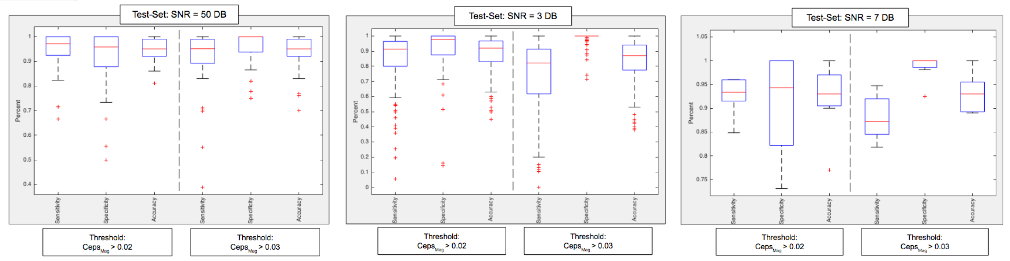
\includegraphics[width=1.6\textwidth]{bilder/all_boxplots.png}
	\caption{Boxplot-Auswertung über Sensitivität, Spezifität und Genauigkeit der beiden besten Modelle}
	\label{img:boxplots}
\end{figure}

\end{landscape}

\end{appendices}
